This section shows the measurements obtained with the TRITIUM-Aveiro 0 prototypes during their installation in the Arrocampo dam, which has been the only prototype installed in Arrocampo dam so far. This prototype was installed and working there for more than four months, from March 27, 2019 to August 18, 2019, during which time this prototype was taking background measurements. The data adquired during this time are shown in the figure \ref{fig:BackgroundArrocampoAveiro}, the measurement time of which is 60 minutes.

\begin{figure}[h]
\centering
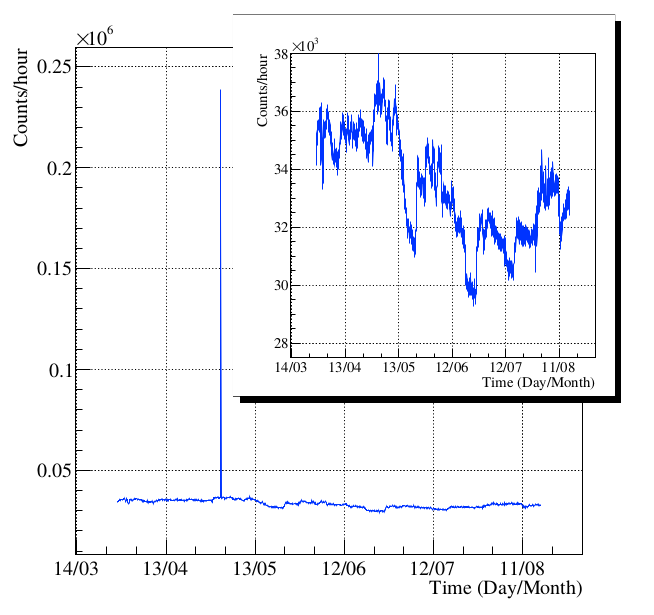
\includegraphics[scale=0.45]{7ExperimentalResultsDetectors/72ExperimentalResultsArrocampo/721TRITIUMAVEIRO0/BackgroundMeasurements.png}
\caption{Background measured with the TRITIUM-Aveiro 0 prototype during its installation in Arrocampo dam \cite{ExperimentalPaperCarlos}.\label{fig:BackgroundArrocampoAveiro}}
\end{figure}

This data shows good stability in the working months, measuring a mean value of around $9.31$ counts per second. A large peak is observed on May 2, 2019, caused by an opening of the roof of the lead shield to access the prototype. In the small box of the figure, the data is zoomed for a better visualization. The MDA measured in Arrocampo dam for 60 minute integration counting data is 6 times larger than that calculated in section \ref{subsec:ResultsTritiumAveiro}. This variations can be caused by electric noise induced by the electric pumps of the water purification system and inestabilities observed in the electronic boards.

A cosmic veto currently under development is planned to be installed and used in anti-coincidence along with two additional prototypes.

Furthermore, three TRITIUM-IFIC 2 prototypes and a cosmic veto, explained in section \ref{subsec:TritiumIFIC2} and \ref{subsec:SetUpActiveShield} respectively, are also planned to be installed in Arrocampo dam as soon as possible.